
\section{Functional Requirements}
    \label{section:functionalReq}
    This section describes the functional requirements for the Archive service.
    The functional aspects which carves the Archive service are mentioned below.

    \subsection{Archive Project Resources}
        The designed system must be able to archive the MARS resources from the active system (Ceph cluster at the time of writing) 
        into the Synology \cite{Synology}. The application must
        be able to archive a project which does not have all the resources mentioned in Table \ref{table: archivedMars} (e.g. no simulation runs have been triggered).
        This must be supported since it could be the case that the user wants to archive only some of the resources.
        
        \begin{table}[H]
            \centering
            \begin{tabular}{|p{3cm}|p{12cm}|}
                \hline
                    \textbf{Resource Name}  & \textbf{Description}\\
                \hline
                     Metadatas & 
                     This resource stores the metadata (e.g. file id, file name). It gives the system the information about
                     existing files in the system. \\
                \hline
                     Files & 
                     This resource correspond to the models (e.g. wolves and sheep model) and input files (e.g. GIS, Time series) which describe a simulation. \\
                \hline
                     Scenarios & 
                     This resource defines the parameters for the model which would be simulated (e.g. simulation run time, number of agents). \\
                \hline
                     Result Configurations & 
                     This resource defines which parameters of a model and layers are going to be stored in the database that will be used for visualization.\\
                \hline
                     Simulation Plans & 
                     This resource contains the scenario and the result configuration which can be executed. The simulation plan could be configured to
                     have different scenario and result configuration to produce different kind of output.\\
                \hline
                     Simulation Runs & 
                     This resource contains the metadata for a simulation results i.e. simulation id, simulation status.\\
                \hline
                     Simulation Results & 
                     This resource is the output and contains the results for a single simulation run.\\
                \hline
            \end{tabular}
            \caption{MARS resources which are to be archived}
            \label{table: archivedMars}     
        \end{table} 
        
        \subsubsection{Assurance of correct data being persisted}
            MARS being a Distributed System, Data Coherency (Subsection \ref{subsection: distriChallenges}) 
            is one of the big issue which this thesis faces. As a consequence,
            wrong or unwanted data could be archived. Therefore the Archive service must ensure that while an archive is running the data would not be
            altered.
        
        \subsection{Retrieve Project Resources}    
            \label{ssec:retrieveAnalysis}
            The designed software must support the retrieval of the archived projects from the Synology into the active system. The
            system must be able to restore the project given that, the services support the data format which is archived in the Synology.
           
            \begin{figure}[H]
                \centering 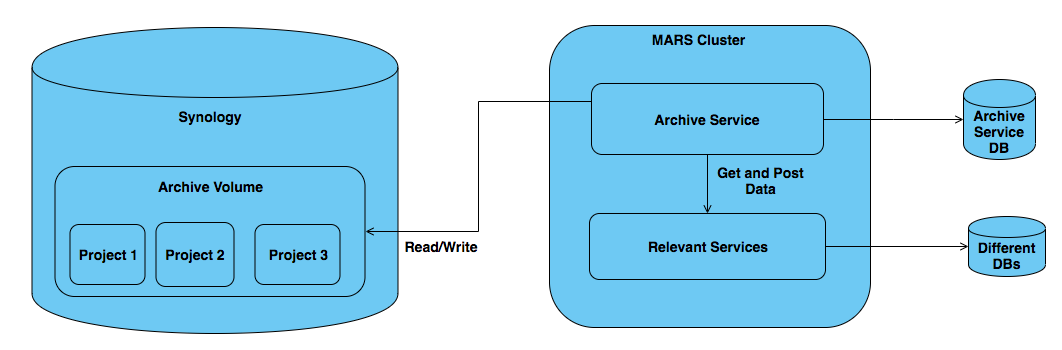
\includegraphics[scale=0.4]{grafiken/synology.png}
                \caption{Archive service's communication structure}
                \label{fig:synology}
            \end{figure}

            Figure \ref{fig:synology} illustrates that the Archive service must only use the volume assigned for archiving and nothing more. 
            This requirement must be fulfilled to comply with the MARS development standard. It has to also be made sure that the retrieved
            resources are usable (e.g. the restored simulation plans should be able to run a simulation again). 

        \subsection{Archive and Retrieve Process Status}  
            The archive and retrieve processes are a long running tasks. The designed software must run these processes in the background to avoid 
            long waiting time for another request. Given this, a API endpoint must be made available which gives the current status of the archive 
            or retrieve job. Using the status a user can determine whether the job is being executed or is finished.


        \subsection{Download Archived Data as a Compressed File}
        \label{sec:anaCompress}
            It is of great importance for a domain Expert i.e. ecologist who are not technical experts to have a graphical interface. In this interface,
            it must be possible to navigate to the project of interest and easily download the project as a zip file. There could be cases where the
            MARS system is out of order and the data is required which could then be accessible by anyone with basic knowledge of the system.
        
        \subsection{Fault-Tolerant Design}   
        Firstly, the Archive service has to communicate with many services in the system, leading the rate of failure being higher
        in comparison to a system which does not depend on other services. A breakdown 
        of one service would cause the whole process of archive/retrieve to stop unexpectedly.  Secondly, it is also possible that a running Archive service be terminated
        due to some unexpected reason. Therefore, fault tolerance mechanism has to be included in the Archive system so that it has a chance of 
        recovery. 
